\documentclass{standalone}
\usepackage{tikz}
\usetikzlibrary{patterns, positioning}

\begin{document}
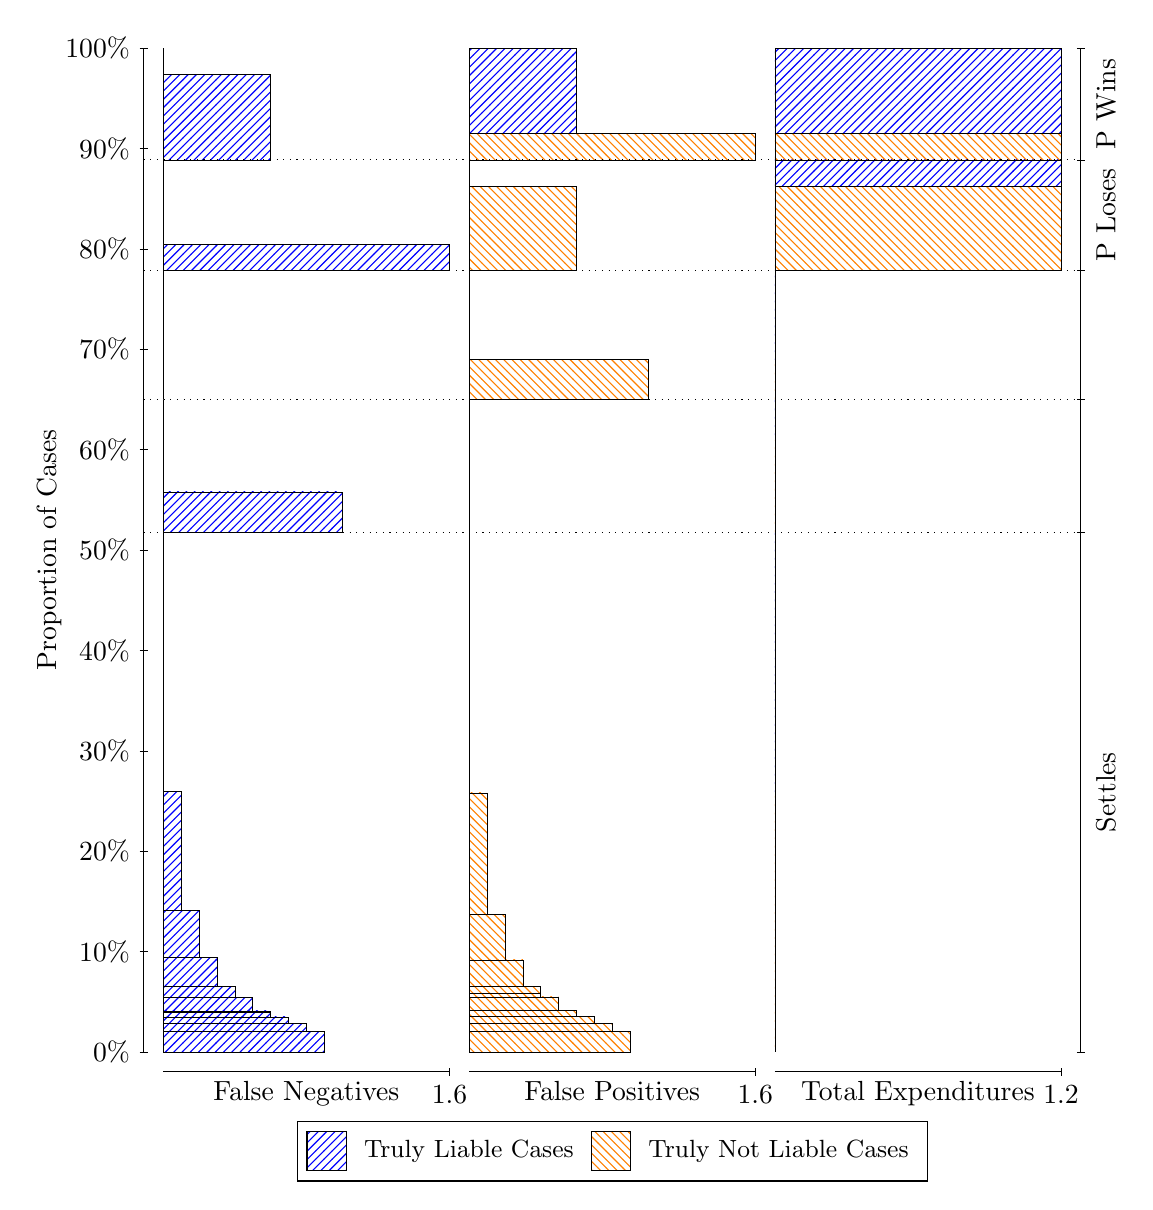
\begin{tikzpicture}
\draw[black, very thin] (1.5,1.75) -- (1.5,14.5);
\node[rotate=90, anchor=center] at (0.3, 8.125) {Proportion of Cases};
\draw[black, very thin] (1.45,1.75) -- (1.55,1.75);
\node[anchor=east] at (1.45, 1.75) {0\%};
\draw[black, very thin] (1.45,3.025) -- (1.55,3.025);
\node[anchor=east] at (1.45, 3.025) {10\%};
\draw[black, very thin] (1.45,4.3) -- (1.55,4.3);
\node[anchor=east] at (1.45, 4.3) {20\%};
\draw[black, very thin] (1.45,5.575) -- (1.55,5.575);
\node[anchor=east] at (1.45, 5.575) {30\%};
\draw[black, very thin] (1.45,6.85) -- (1.55,6.85);
\node[anchor=east] at (1.45, 6.85) {40\%};
\draw[black, very thin] (1.45,8.125) -- (1.55,8.125);
\node[anchor=east] at (1.45, 8.125) {50\%};
\draw[black, very thin] (1.45,9.4) -- (1.55,9.4);
\node[anchor=east] at (1.45, 9.4) {60\%};
\draw[black, very thin] (1.45,10.675) -- (1.55,10.675);
\node[anchor=east] at (1.45, 10.675) {70\%};
\draw[black, very thin] (1.45,11.95) -- (1.55,11.95);
\node[anchor=east] at (1.45, 11.95) {80\%};
\draw[black, very thin] (1.45,13.225) -- (1.55,13.225);
\node[anchor=east] at (1.45, 13.225) {90\%};
\draw[black, very thin] (1.45,14.5) -- (1.55,14.5);
\node[anchor=east] at (1.45, 14.5) {100\%};

\draw[black, very thin] (13.4,1.75) -- (13.4,14.5);
\draw[black, very thin] (13.35,1.75) -- (13.45,1.75);
\node[anchor=west] at (13.35, 1.75) {};
\draw[black, very thin] (13.35,8.35) -- (13.45,8.35);
\node[anchor=west] at (13.35, 8.35) {};
\draw[black, very thin] (13.35,10.037) -- (13.45,10.037);
\node[anchor=west] at (13.35, 10.037) {};
\draw[black, very thin] (13.35,11.673) -- (13.45,11.673);
\node[anchor=west] at (13.35, 11.673) {};
\draw[black, very thin] (13.35,13.08) -- (13.45,13.08);
\node[anchor=west] at (13.35, 13.08) {};
\draw[black, very thin] (13.35,14.5) -- (13.45,14.5);
\node[anchor=west] at (13.35, 14.5) {};

\draw[black, very thin, pattern color=blue, pattern=north east lines] (1.75,1.75) rectangle (3.7937,2.0153);
\draw[black, very thin, pattern color=blue, pattern=north east lines] (1.75,2.0153) rectangle (3.5667,2.1124);
\draw[black, very thin, pattern color=blue, pattern=north east lines] (1.75,2.1124) rectangle (3.3396,2.1952);
\draw[black, very thin, pattern color=blue, pattern=north east lines] (1.75,2.1952) rectangle (3.1125,2.253);
\draw[black, very thin, pattern color=blue, pattern=north east lines] (1.75,2.253) rectangle (3.1125,2.2729);
\draw[black, very thin, pattern color=blue, pattern=north east lines] (1.75,2.2729) rectangle (2.8854,2.4464);
\draw[black, very thin, pattern color=blue, pattern=north east lines] (1.75,2.4464) rectangle (2.6583,2.5802);
\draw[black, very thin, pattern color=blue, pattern=north east lines] (1.75,2.5802) rectangle (2.4312,2.9466);
\draw[black, very thin, pattern color=blue, pattern=north east lines] (1.75,2.9466) rectangle (2.2042,3.5504);
\draw[black, very thin, pattern color=blue, pattern=north east lines] (1.75,3.5504) rectangle (1.9771,5.06);
\draw[black, very thin, pattern color=orange, pattern=north west lines] (1.75,5.06) rectangle (1.75,8.35);
\draw[black, very thin, pattern color=blue, pattern=north east lines] (1.75,8.35) rectangle (4.0208,8.8632);
\draw[black, very thin, pattern color=orange, pattern=north west lines] (1.75,8.8632) rectangle (1.75,10.037);
\draw[black, very thin, pattern color=orange, pattern=north west lines] (1.75,10.037) rectangle (1.75,10.541);
\draw[black, very thin, pattern color=blue, pattern=north east lines] (1.75,10.541) rectangle (1.75,11.673);
\draw[black, very thin, pattern color=blue, pattern=north east lines] (1.75,11.673) rectangle (5.3833,12.007);
\draw[black, very thin, pattern color=orange, pattern=north west lines] (1.75,12.007) rectangle (1.75,13.08);
\draw[black, very thin, pattern color=blue, pattern=north east lines] (1.75,13.08) rectangle (3.1125,14.166);
\draw[black, very thin, pattern color=orange, pattern=north west lines] (1.75,14.166) rectangle (1.75,14.5);
\draw[black, very thin, pattern color=orange, pattern=north west lines] (5.6333,1.75) rectangle (7.6771,2.0139);
\draw[black, very thin, pattern color=orange, pattern=north west lines] (5.6333,2.0139) rectangle (7.45,2.1157);
\draw[black, very thin, pattern color=orange, pattern=north west lines] (5.6333,2.1157) rectangle (7.2229,2.2052);
\draw[black, very thin, pattern color=orange, pattern=north west lines] (5.6333,2.2052) rectangle (6.9958,2.2809);
\draw[black, very thin, pattern color=orange, pattern=north west lines] (5.6333,2.2809) rectangle (6.7687,2.4509);
\draw[black, very thin, pattern color=orange, pattern=north west lines] (5.6333,2.4509) rectangle (6.5417,2.4949);
\draw[black, very thin, pattern color=orange, pattern=north west lines] (5.6333,2.4949) rectangle (6.5417,2.5832);
\draw[black, very thin, pattern color=orange, pattern=north west lines] (5.6333,2.5832) rectangle (6.3146,2.9191);
\draw[black, very thin, pattern color=orange, pattern=north west lines] (5.6333,2.9191) rectangle (6.0875,3.4986);
\draw[black, very thin, pattern color=orange, pattern=north west lines] (5.6333,3.4986) rectangle (5.8604,5.04);
\draw[black, very thin, pattern color=blue, pattern=north east lines] (5.6333,5.04) rectangle (5.6333,8.35);
\draw[black, very thin, pattern color=orange, pattern=north west lines] (5.6333,8.35) rectangle (5.6333,9.524);
\draw[black, very thin, pattern color=blue, pattern=north east lines] (5.6333,9.524) rectangle (5.6333,10.037);
\draw[black, very thin, pattern color=orange, pattern=north west lines] (5.6333,10.037) rectangle (7.9042,10.541);
\draw[black, very thin, pattern color=blue, pattern=north east lines] (5.6333,10.541) rectangle (5.6333,11.673);
\draw[black, very thin, pattern color=orange, pattern=north west lines] (5.6333,11.673) rectangle (6.9958,12.746);
\draw[black, very thin, pattern color=blue, pattern=north east lines] (5.6333,12.746) rectangle (5.6333,13.08);
\draw[black, very thin, pattern color=orange, pattern=north west lines] (5.6333,13.08) rectangle (9.2667,13.414);
\draw[black, very thin, pattern color=blue, pattern=north east lines] (5.6333,13.414) rectangle (6.9958,14.5);
\draw[black, very thin, pattern color=orange, pattern=north west lines] (9.5167,1.75) rectangle (9.5167,5.04);
\draw[black, very thin, pattern color=blue, pattern=north east lines] (9.5167,5.04) rectangle (9.5167,8.35);
\draw[black, very thin, pattern color=orange, pattern=north west lines] (9.5167,8.35) rectangle (9.5167,9.524);
\draw[black, very thin, pattern color=blue, pattern=north east lines] (9.5167,9.524) rectangle (9.5167,10.037);
\draw[black, very thin, pattern color=orange, pattern=north west lines] (9.5167,10.037) rectangle (9.5167,10.541);
\draw[black, very thin, pattern color=blue, pattern=north east lines] (9.5167,10.541) rectangle (9.5167,11.673);
\draw[black, very thin, pattern color=orange, pattern=north west lines] (9.5167,11.673) rectangle (13.15,12.746);
\draw[black, very thin, pattern color=blue, pattern=north east lines] (9.5167,12.746) rectangle (13.15,13.08);
\draw[black, very thin, pattern color=orange, pattern=north west lines] (9.5167,13.08) rectangle (13.15,13.414);
\draw[black, very thin, pattern color=blue, pattern=north east lines] (9.5167,13.414) rectangle (13.15,14.5);
\draw[black, dotted] (1.5,8.35) -- (13.4,8.35);
\draw[black, dotted] (1.5,10.037) -- (13.4,10.037);
\draw[black, dotted] (1.5,11.673) -- (13.4,11.673);
\draw[black, dotted] (1.5,13.08) -- (13.4,13.08);
\draw[black, very thin] (1.75,1.5) -- (5.3833,1.5);
\node[anchor=north] at (3.5667, 1.5) {False Negatives};
\draw[black, very thin] (5.3833,1.45) -- (5.3833,1.55);
\node[anchor=north] at (5.3833, 1.45) {1.6};

\draw[black, very thin] (5.6333,1.5) -- (9.2667,1.5);
\node[anchor=north] at (7.45, 1.5) {False Positives};
\draw[black, very thin] (9.2667,1.45) -- (9.2667,1.55);
\node[anchor=north] at (9.2667, 1.45) {1.6};

\draw[black, very thin] (9.5167,1.5) -- (13.15,1.5);
\node[anchor=north] at (11.333, 1.5) {Total Expenditures};
\draw[black, very thin] (13.15,1.45) -- (13.15,1.55);
\node[anchor=north] at (13.15, 1.45) {1.2};

\node[black, centered, rotate=90] at (13.72, 5.05) {Settles};


\node[black, centered, rotate=90] at (13.72, 12.376) {P Loses};
\node[black, centered, rotate=90] at (13.72, 13.79) {P Wins};

\draw (7.449999999999999,1.5) node[draw=none] (baseCoordinate) {};
\begin{scope}[align=center]
        \matrix[scale=0.5, draw=black, below=0.5cm of baseCoordinate, nodes={draw}, column sep=0.1cm]{
            \node[rectangle, draw, minimum width=0.5cm, minimum height=0.5cm, pattern=north east lines, pattern color=blue] {}; &
            \node[draw=none, font=\small] (B) {Truly Liable Cases}; &
            \node[rectangle, draw, minimum width=0.5cm, minimum height=0.5cm, pattern=north west lines, pattern color=orange] {}; &
            \node[draw=none, font=\small] (B) {Truly Not Liable Cases}; \\
            };
\end{scope}

\end{tikzpicture}
\end{document}